\documentclass[14pt,a4paper,oneside]{extarticle}

\usepackage[utf8]{inputenc}
\usepackage[T2A]{fontenc}
\usepackage[ukrainian]{babel}

%% --- Оформлення за вимогами ДСТУ 3008--95 (структура звіту, поля, інтервал, абзац) ---
%% Примітка: гарнітура Times New Roman у pdfLaTeX потребує окремих пакетів/шрифтів;
%% за замовчуванням --- стандартні T2A-шрифти (читабельний вигляд для здачі).
\usepackage[a4paper,left=30mm,right=15mm,top=20mm,bottom=20mm]{geometry}
\usepackage{setspace}
\onehalfspacing
\usepackage{indentfirst}
\setlength{\parindent}{1.25cm}

\usepackage{amsmath}
\usepackage{amssymb}
\usepackage{float}
\usepackage{array}
\usepackage{tabularx}
\usepackage{graphicx}
\usepackage{caption}
\usepackage{subcaption}
\DeclareCaptionLabelSeparator{dstudash}{\,---\,}
\captionsetup{format=plain,labelfont=bf,labelsep=dstudash}
\captionsetup[figure]{justification=centering}
%% Таблиці за ДСТУ: підпис зверху, вирівнювання зліва; без booktabs --- повна сітка ліній
\captionsetup[table]{position=top,justification=raggedright,singlelinecheck=false}

\addto\captionsukrainian{%
  \renewcommand{\figurename}{Рисунок}%
  \renewcommand{\tablename}{Таблиця}%
  \renewcommand{\refname}{Список використаних джерел}%
  \renewcommand{\abstractname}{Анотація}%
  \renewcommand{\contentsname}{Зміст}%
}

%% Посилання: квадратні дужки [1] (звична форма для робіт за ДСТУ)
\usepackage[numbers,square,sort&compress]{natbib}
\usepackage[hidelinks]{hyperref}
\usepackage{url}

\setcounter{secnumdepth}{3}
\setcounter{tocdepth}{3}

\graphicspath{{figures/}}

\begin{document}

%% ---------- Титульний аркуш (реквізити як у лабораторних звітах lab1/lab3) ----------
\begin{titlepage}
\thispagestyle{empty}
\begin{center}
{\Large \textbf{КИЇВСЬКИЙ НАЦІОНАЛЬНИЙ УНІВЕРСИТЕТ\\
ІМЕНІ ТАРАСА ШЕВЧЕНКА}}\\[2\baselineskip]
{\large Факультет комп'ютерних наук та кібернетики}\\[3\baselineskip]
{\Large \textbf{РЕФЕРАТ}}\\[0.75\baselineskip]
{\normalsize з дисципліни «Методи негладкої оптимізації»}\\[2.5\baselineskip]
{\normalsize на тему:}\\[0.75\baselineskip]
{\large \textbf{Феноменологія та прикладні аспекти стохастичних фракталів у сучасній науці та інженерії:\\від процедурної генерації до фінансового моделювання}}\\[4\baselineskip]
\end{center}
\begin{flushright}
Виконав:\\[0.25\baselineskip]
студент групи ПМ\\[0.4\baselineskip]
{\Large \textbf{Кіщук Ярослав Ярославович}}\\[2\baselineskip]
\end{flushright}
\vfill
\begin{center}
{\large \textbf{Київ --- 2026}}
\end{center}
\end{titlepage}
\clearpage

\begin{abstract}
Розглянуто перехід від евклідової геометрії до фрактальної парадигми, роль стохастичних компонент у самоподібних структурах та прикладні галузі: комп'ютерна графіка й ландшафти, фрактальне стиснення зображень, біологія й медицина, фрактальні антени, гіпотеза фрактального ринку, дифузійно-обмежена агрегація, стохастичний фрактальний пошук, метеорологія.
\end{abstract}
\clearpage

\tableofcontents
\clearpage

% Порядок у списку літератури відповідає заданій нумерації c01--c46
\nocite{c01,c02,c03,c04,c05,c06,c07,c08,c09,c10,c11,c12,c13,c14,c15,c16,c17,c18,c19,c20,c21,c22,c23,c24,c25,c26,c27,c28,c29,c30,c31,c32,c33,c34,c35,c36,c37,c38,c39,c40,c41,c42,c43,c44,c45,c46,c47,c52}

\section{Вступ}
Розвиток сучасної наукової думки наприкінці XX століття ознаменувався фундаментальним переходом від ідеалізованих евклідових форм до розуміння глибокої впорядкованості хаосу. Традиційна геометрія, що оперує цілочисельними вимірами, виявилася неспроможною адекватно описати морфологію природних об'єктів --- від порізаних берегових ліній до структури людських легень.\cite{c01}
Введення Бенуа Мандельбротом поняття фракталу --- структури, що демонструє самоподібність на різних масштабах --- відкрило нову еру в моделюванні складних систем.\cite{c02,c45}
Особливу цінність для прикладної науки становлять стохастичні фрактали, де до строгих алгоритмів самоподібності додаються випадкові компоненти, що дозволяє створювати моделі, статистично близькі до природних явищ.\cite{c04}

\section{Теоретичний базис та математична природа фрактальних об'єктів}
У самому серці фрактальної геометрії лежить концепція рекурсії та нескінченної деталізації. Фрактал можна визначити як геометричну конструкцію, що виявляє складність на будь-якому рівні збільшення.\cite{c05}
На відміну від об'єктів евклідової геометрії, які при масштабуванні втрачають деталі (наприклад, коло при сильному збільшенні виглядає як пряма лінія), фрактали зберігають або навіть нарощують свою складність.\cite{c05}
Кількісною мірою цієї складності є фрактальна розмірність ($D$), яка зазвичай є дробовим числом.\cite{c02}

Математично фрактальна розмірність визначається через співвідношення між зміною масштабу та кількістю нових елементів, що з'являються. Для ідеально самоподібного об'єкта, де ціле складається з $N$ копій самого себе, зменшених у $s$ разів, розмірність обчислюється за формулою
\begin{equation}
  D = \frac{\ln N}{\ln(1/s)}.
\end{equation}
Наприклад, для кривої Коха, де кожна лінія замінюється чотирма сегментами довжиною в одну третину від оригіналу ($N=4$, $s=1/3$), розмірність становить $D \approx 1{,}2619$.\cite{c02}
Це вказує на те, що крива Коха є «більшою» за одновимірну лінію, але ще не досягає властивостей двовимірної площини.\cite{c05}
У фізичному світі такий підхід дозволяє оцінювати шорсткість поверхонь, що важливо для аналізу зносу деталей або прогнозування тертя в механічних системах.\cite{c02}

\begin{figure}[H]
  \centering
  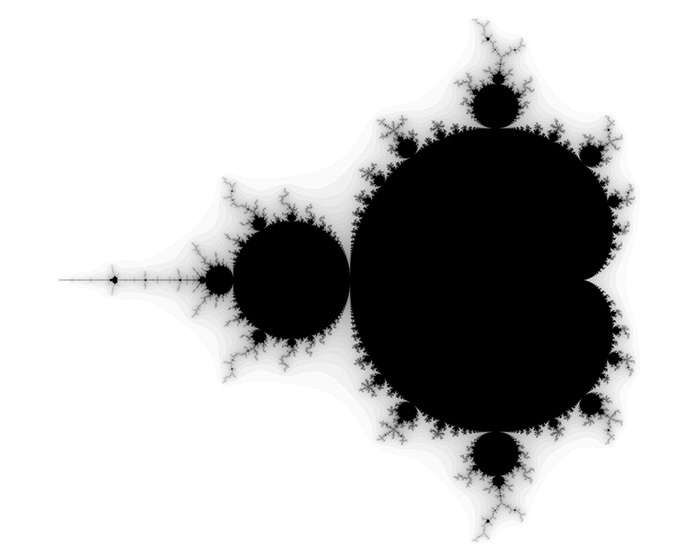
\includegraphics[width=\linewidth,height=0.46\textheight,keepaspectratio]{external/ext_mandelbrot.jpg}
  \caption{Класичний фрактал Мандельброта (фрагмент множини): на межі хаосу й порядку структура лишається деталізованою при зміні масштабу. Ілюстрація з матеріалів {Paul Bourke}\cite{c47}.}
  \label{fig:extmandel}
\end{figure}

\section{Порівняльна характеристика детермінованих та стохастичних моделей}
Розуміння різниці між детермінованими та стохастичними фракталами є ключовим для їх практичного застосування. Детерміновані системи виробляють фіксований вихід для кожного входу, не залишаючи місця для випадковості.\cite{c05}
Стохастичні ж моделі включають елементи ймовірності, що дозволяє їм краще імітувати непередбачуваність реального світу.\cite{c04}

\begin{table}[H]
  \centering
  \renewcommand{\arraystretch}{1.15}
  \caption{Порівняння детермінованих і стохастичних фракталів (узагальнено за\cite{c05,c07,c08,c10})}
  \begin{tabularx}{\textwidth}{|>{\raggedright\arraybackslash}X|>{\raggedright\arraybackslash}X|>{\raggedright\arraybackslash}X|}
    \hline
    \textbf{Критерій} & \textbf{Детерміновані фрактали} & \textbf{Стохастичні фрактали} \\
    \hline
    Природа генерації & Суворі математичні правила без випадковості.\cite{c05} & Використання ГПВЧ у процесі ітерації.\cite{c05} \\
    \hline
    Тип самоподібності & Строга геометрична самоподібність. & Статистична самоподібність.\cite{c02} \\
    \hline
    Візуальний вигляд & Ідеальні симетричні паттерни (наприклад, трикутник Серпінського).\cite{c05} & Природні хаотичні форми (ландшафти, хмари, фінансові ряди).\cite{c04} \\
    \hline
    Прогнозованість & Повністю передбачуваний результат.\cite{c07} & Результат варіюється; моделювання невизначеності.\cite{c08} \\
    \hline
    Математична основа & Ітераційні функціональні системи (IFS).\cite{c11} & Фрактальний броунівський рух (fBm), шум $1/f$.\cite{c05} \\
    \hline
  \end{tabularx}
  \renewcommand{\arraystretch}{1.0}
\end{table}

\begin{figure}[H]
  \centering
  
\includegraphics[width=\linewidth,height=0.34\textheight,keepaspectratio]{external/ext_sierpinski.png}
  \caption{Трикутник Серпінського як канонічний приклад строгої геометричної самоподібності (ітераційна побудова). Ілюстрація з блогу {JEM Engineering}\cite{c09}.}
  \label{fig:extsierp}
\end{figure}

\begin{figure}[H]
  \centering
  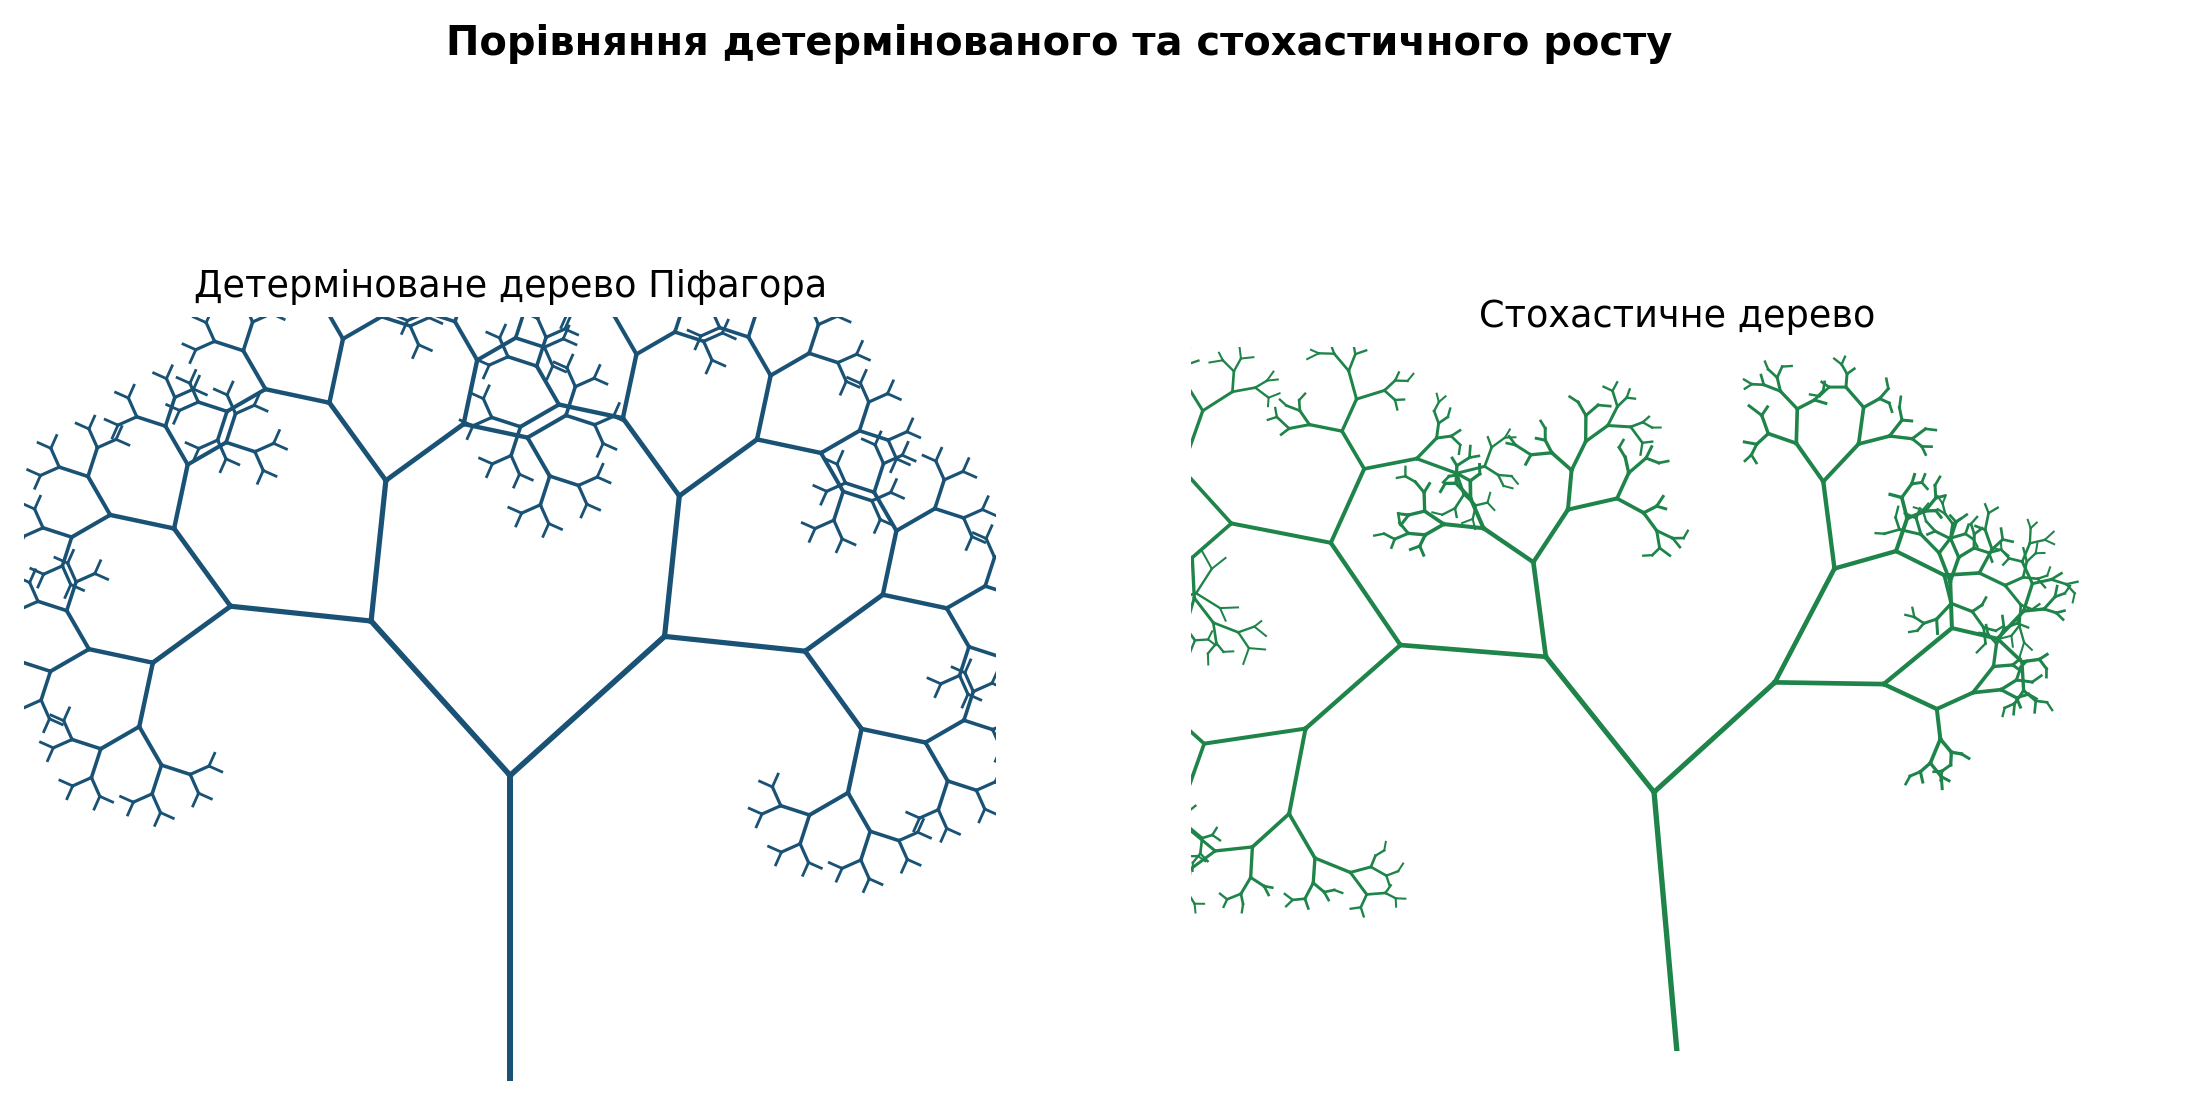
\includegraphics[width=\linewidth]{fig01_trees.png}
  \caption{Порівняльна візуалізація детермінованого (дерево Піфагора) та стохастичного росту (випадкові кути й довжини гілок). Згенеровано Python.}
  \label{fig:trees}
\end{figure}

\section{Стохастичне моделювання в комп'ютерній графіці та ландшафтах}
Однією з найперших і найуспішніших сфер застосування стохастичних фракталів стала комп'ютерна графіка: замість явного опису кожної деталі задають алгоритм росту, який породжує високу деталізацію.\cite{c02,c05}

\subsection{Алгоритми випадкового зміщення та рельєф}
Фундаментальним інструментом для реалістичних гір і долин є випадкове зміщення середньої точки (RMD); відома реалізація --- Diamond--Square на квадратній сітці.\cite{c14,c12}
Етапи: ініціалізація висот у кутах; крок \emph{diamond} (центр квадрата); крок \emph{square} (центри ромбів); рекурсія зі зменшенням амплітуди шуму, зокрема пропорційно $2^{-h}$, де $h$ керує «шорсткістю» ландшафту ($0 \le h \le 1$).\cite{c14}
Метод реалізований у численних пакетах і навчальних репозиторіях.\cite{c12}
Незважаючи на простоту, такі алгоритми дають переконливі моделі рельєфу й використовуються в індустріальних пайплайнах процедурної графіки; водночас можливі лінійні артефакти («крейдяні лінії»), що мотивує перехід до градієнтних шумів.\cite{c14}
Для більшої органічності застосовують шум Перліна та Simplex noise; накладання октав дає фрактальний ландшафт і текстури.\cite{c16,c17,c18}

\section{Фрактальне кодування та стиснення зображень (FIC)}
Технологія FIC спирається на надлишковість самоподібних паттернів у реальних зображеннях; класичним тестовим прикладом лишається зображення Lenna з бази {USC}-{SIPI} (коректне цитування джерела дозволяє використовувати його в навчальних ілюстраціях).\cite{c20,c11,c46}
Етапи: партиціювання на блоки діапазону (range); пошук схожих доменних блоків (domain) більшого розміру; підбір афінних перетворень (контраст, яскравість, геометрія); зберігання «фрактальних кодів» замість сирих пікселів.\cite{c11,c20,c22,c23}
Перевага --- можливість масштабованої декомпресії («фрактальний зум») завдяки збереженій самоподібності; у літературі згадують високі коефіцієнти стиснення для класів текстурованих зображень.\cite{c11,c22}

\begin{figure}[H]
  \centering
  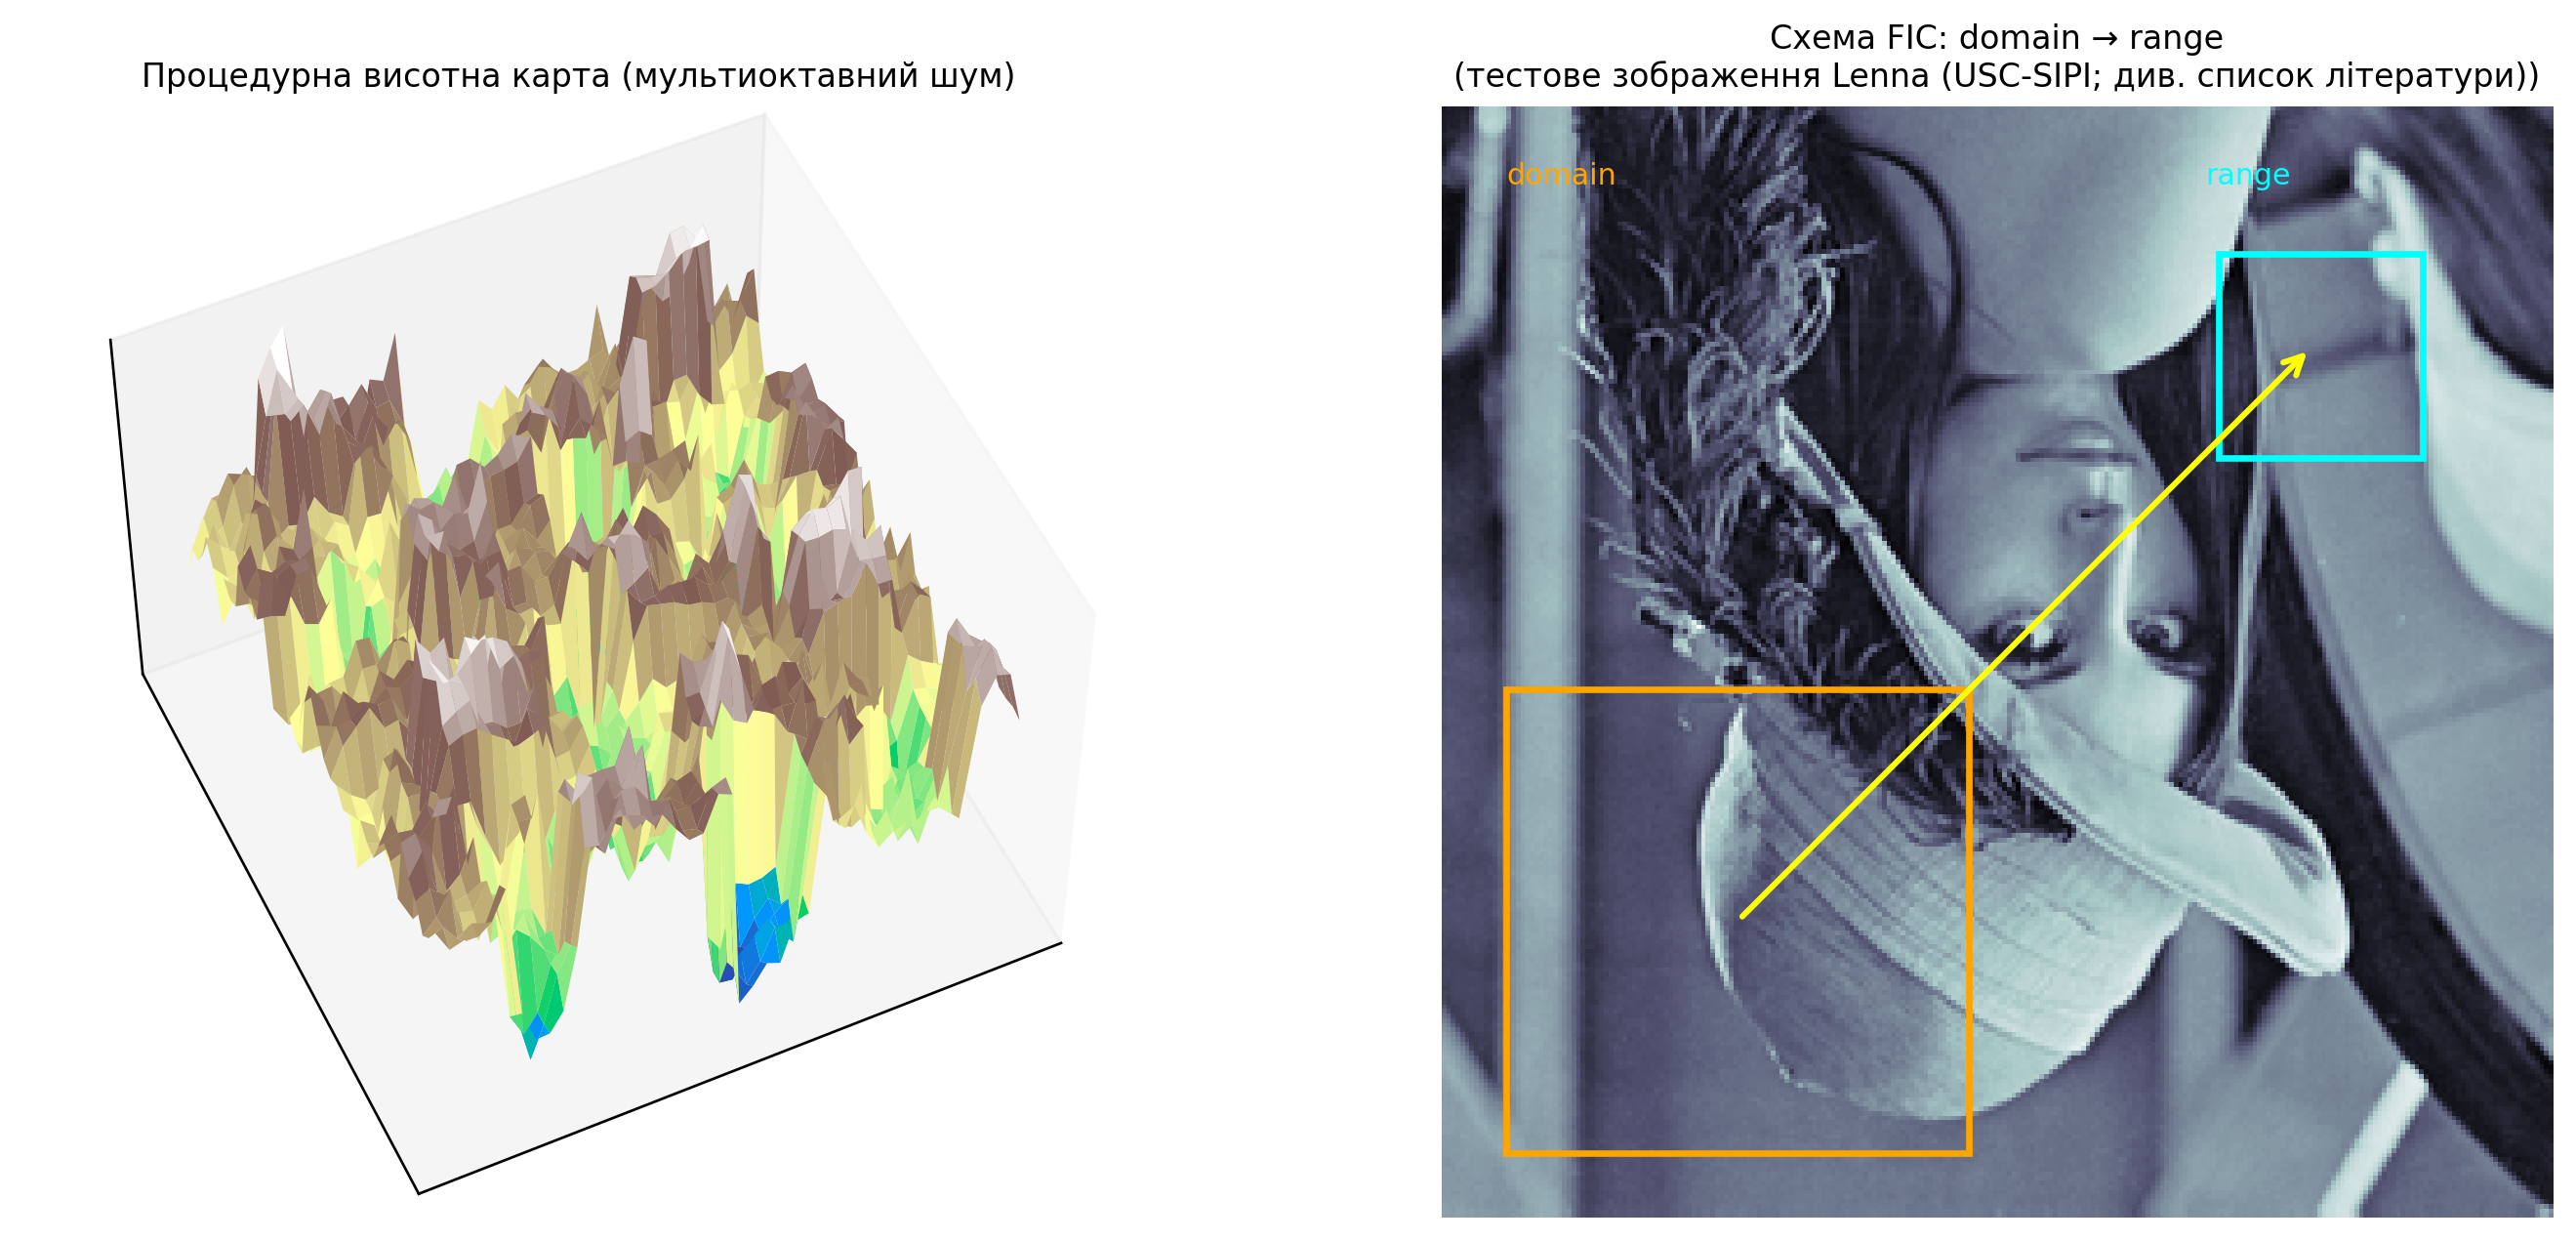
\includegraphics[width=\linewidth]{fig02_landscape_fic.png}
  \caption{Процедурна висотна карта (мультиоктавний шум) як аналог simplex-ландшафту; праворуч --- схематичне фрактальне кодування на тестовому зображенні Lenna з посиланням на базу {USC}-{SIPI}\cite{c46}.}
  \label{fig:landfic}
\end{figure}

\section{Фрактальна архітектура біологічних систем та медицина}
Природа широко використовує фрактальні принципи для транспорту речовин та оптимізації поверхонь.\cite{c24,c25}
Людське тіло поєднує детерміновані генетичні правила зі стохастичним ростом.\cite{c26,c27}

\subsection{Легені та судини}
Бронхіальне дерево забезпечує величезну площу газообміну в обмеженому об'ємі грудної клітки (порядку десятків---сотень м$^2$ при об'ємі кількох літрів).\cite{c28,c26}
Капілярна мережа забезпечує доступ кисню до тканин; фрактальна організація судин супроводжується масштабним сумарним протяженням мережі (у популяризаціях наводять порядки $10^5$ км для дорослого організму як наслідок ієрархічного розгалуження).\cite{c27,c26}

\begin{figure}[H]
  \centering
  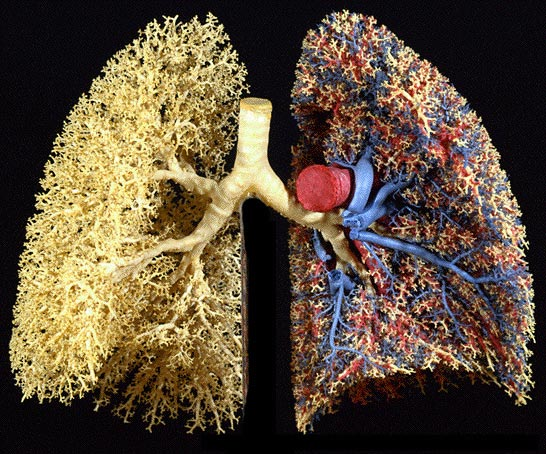
\includegraphics[width=\linewidth,height=0.58\textheight,keepaspectratio]{external/ext_lungs.jpg}
  \caption{Схематичне зображення бронхіального дерева як приклад розгалуженої структури в обмеженому об'ємі (навчальний матеріал {Fractal Foundation})\cite{c25}.}
  \label{fig:extroman}
\end{figure}

\subsection{Нейрони та діагностика}
Мозок демонструє фрактальне розгалуження зв'язків; аналіз фрактальної розмірності (FD) застосовують в онкології (ангіогенез), нейродегенерації, офтальмології.\cite{c29,c26,c27}

\begin{figure}[H]
  \centering
  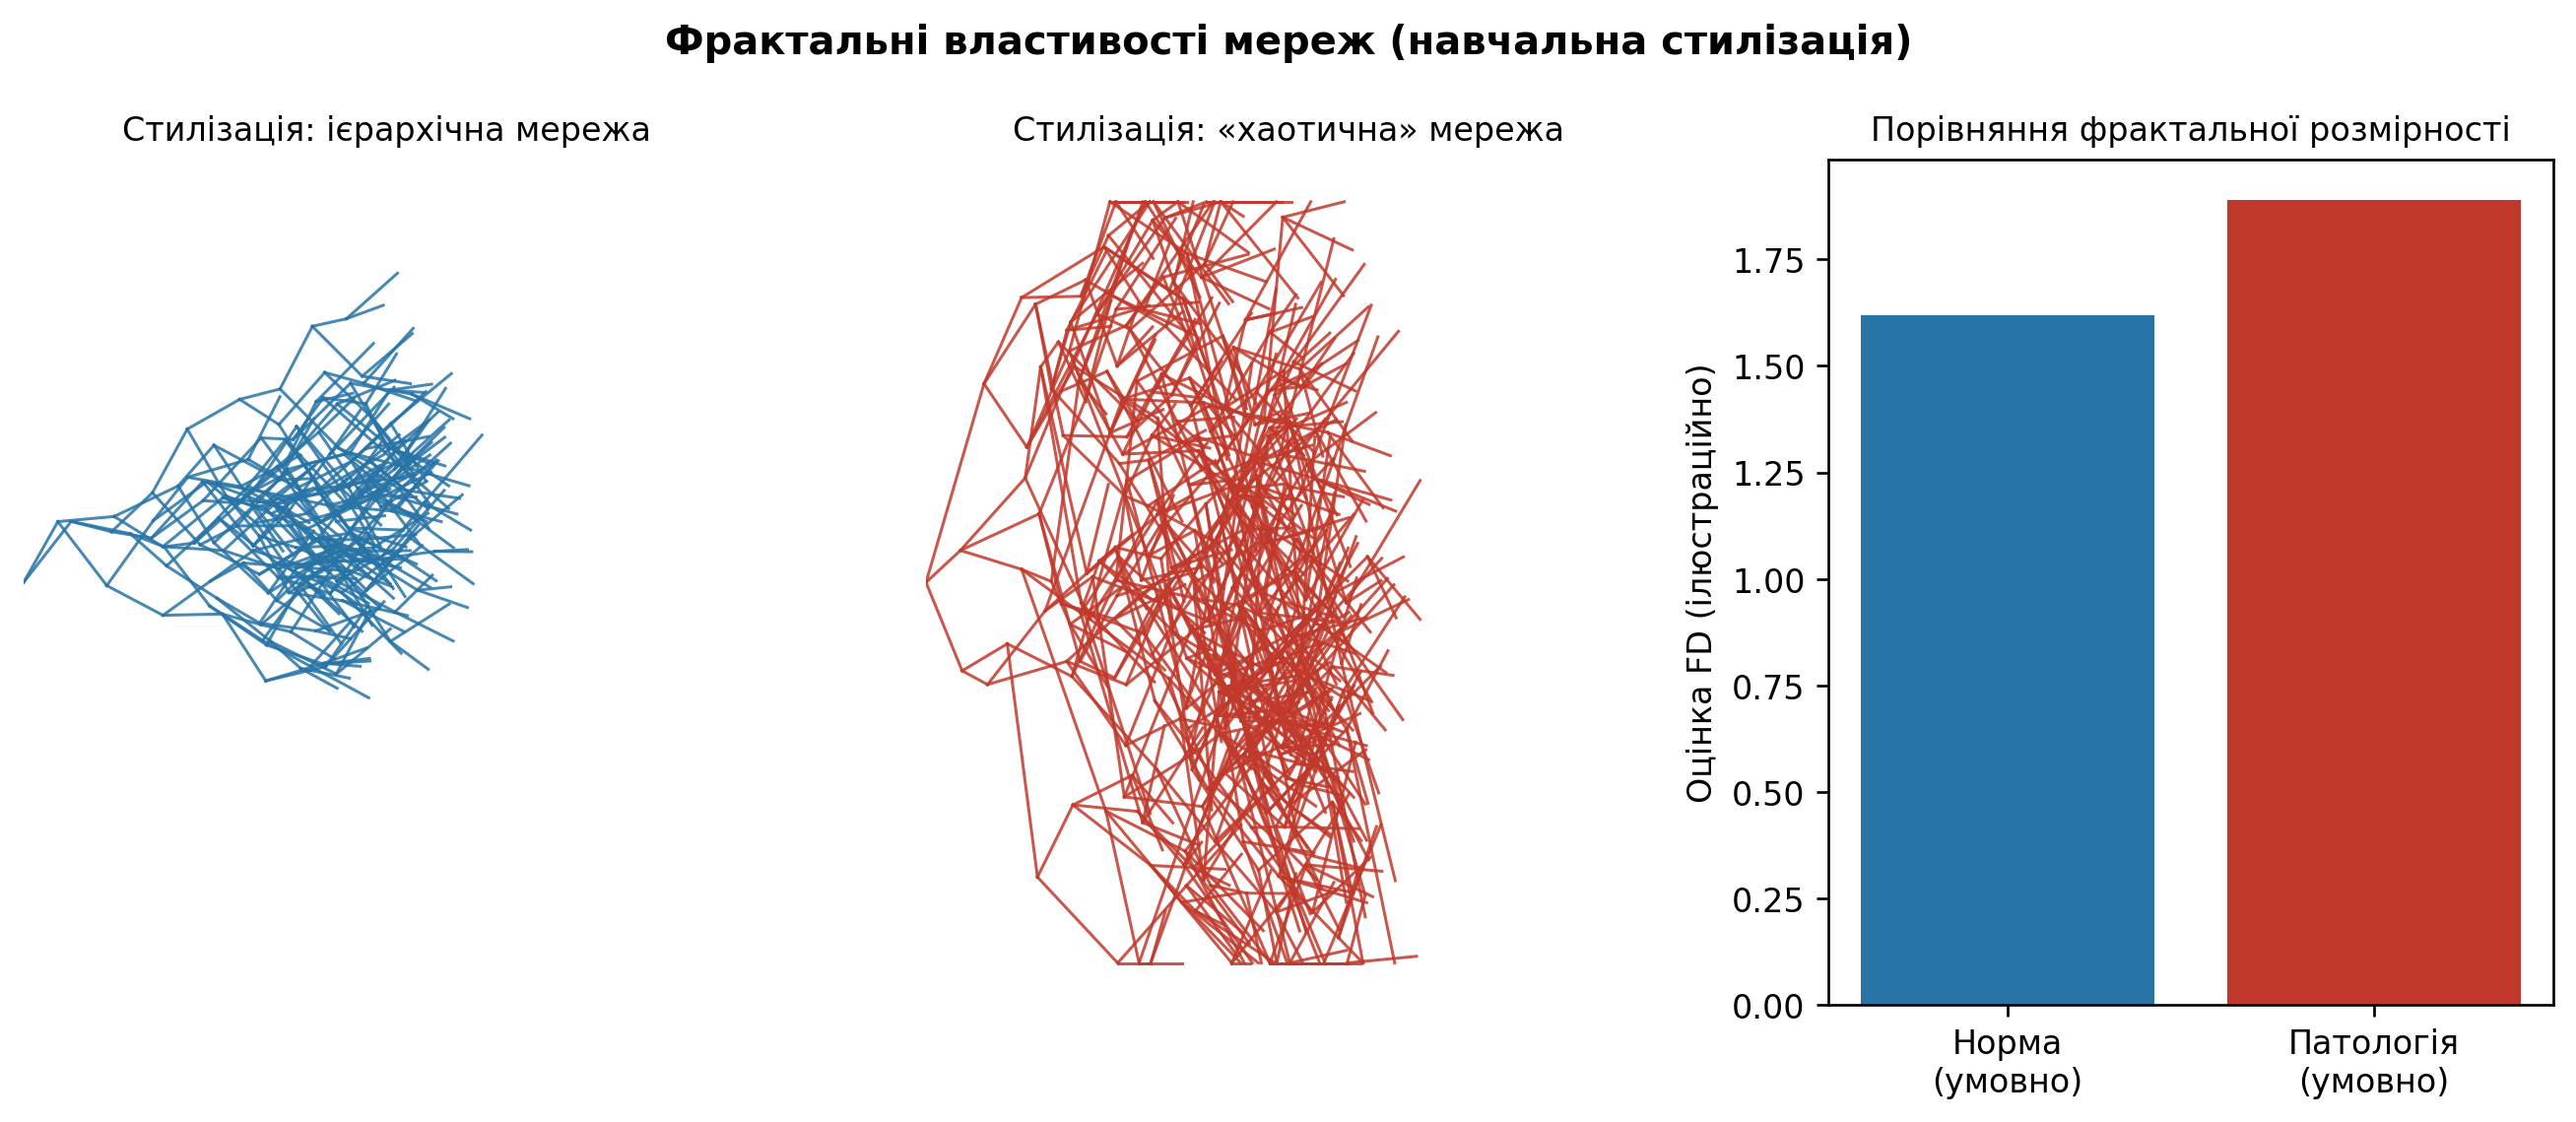
\includegraphics[width=\linewidth]{fig03_vessels_fd.png}
  \caption{Стилізовані мережі: «регулярна» проти «хаотичної» та умовні значення FD (навчальна демонстрація, не клінічні дані).}
  \label{fig:vessels}
\end{figure}

\section{Фрактальні антени: мініатюризація та багатодіапазонність}
У телекомунікаціях фрактальні криві дозволяють упаковувати ефективну довжину провідника в обмежений об'єм (space-filling curves: Гільберта, Коха тощо).\cite{c03,c09,c30,c31}
Переваги: мініатюризація (орієнтовно менший габарит при тій же резонансній частоті), багатодіапазонність завдяки самоподібності масштабів.\cite{c09,c32,c30}
Логарифмічно-періодичні антени історично також розглядають через масштабну інваріантність.\cite{c03,c32}

\begin{table}[H]
  \centering
  \renewcommand{\arraystretch}{1.15}
  \caption{Приклади фракталів у конструкціях антен (за\cite{c09,c30,c31,c03})}
  \small
  \begin{tabularx}{\textwidth}{|>{\raggedright\arraybackslash}X|>{\raggedright\arraybackslash}X|>{\raggedright\arraybackslash}X|}
    \hline
    \textbf{Тип} & \textbf{Застосування} & \textbf{Характеристики} \\
    \hline
    Трикутник Серпінського & Багатодіапазонні патч-антени.\cite{c09} & Частоти, пов'язані з масштабами самоподібності.\cite{c30} \\
    \hline
    Крива Коха & Дипольні та монопольні антени.\cite{c09} & Скорочення фізичної довжини при резонансі.\cite{c09} \\
    \hline
    Килим Серпінського & Планарні решітки.\cite{c30} & Підсилення та спрямованість.\cite{c30} \\
    \hline
    Крива Мінковського & Компактні друковані антени.\cite{c03} & Ефективне заповнення площі субстрату.\cite{c03} \\
    \hline
  \end{tabularx}
  \renewcommand{\arraystretch}{1.0}
\end{table}

\begin{figure}[H]
  \centering
  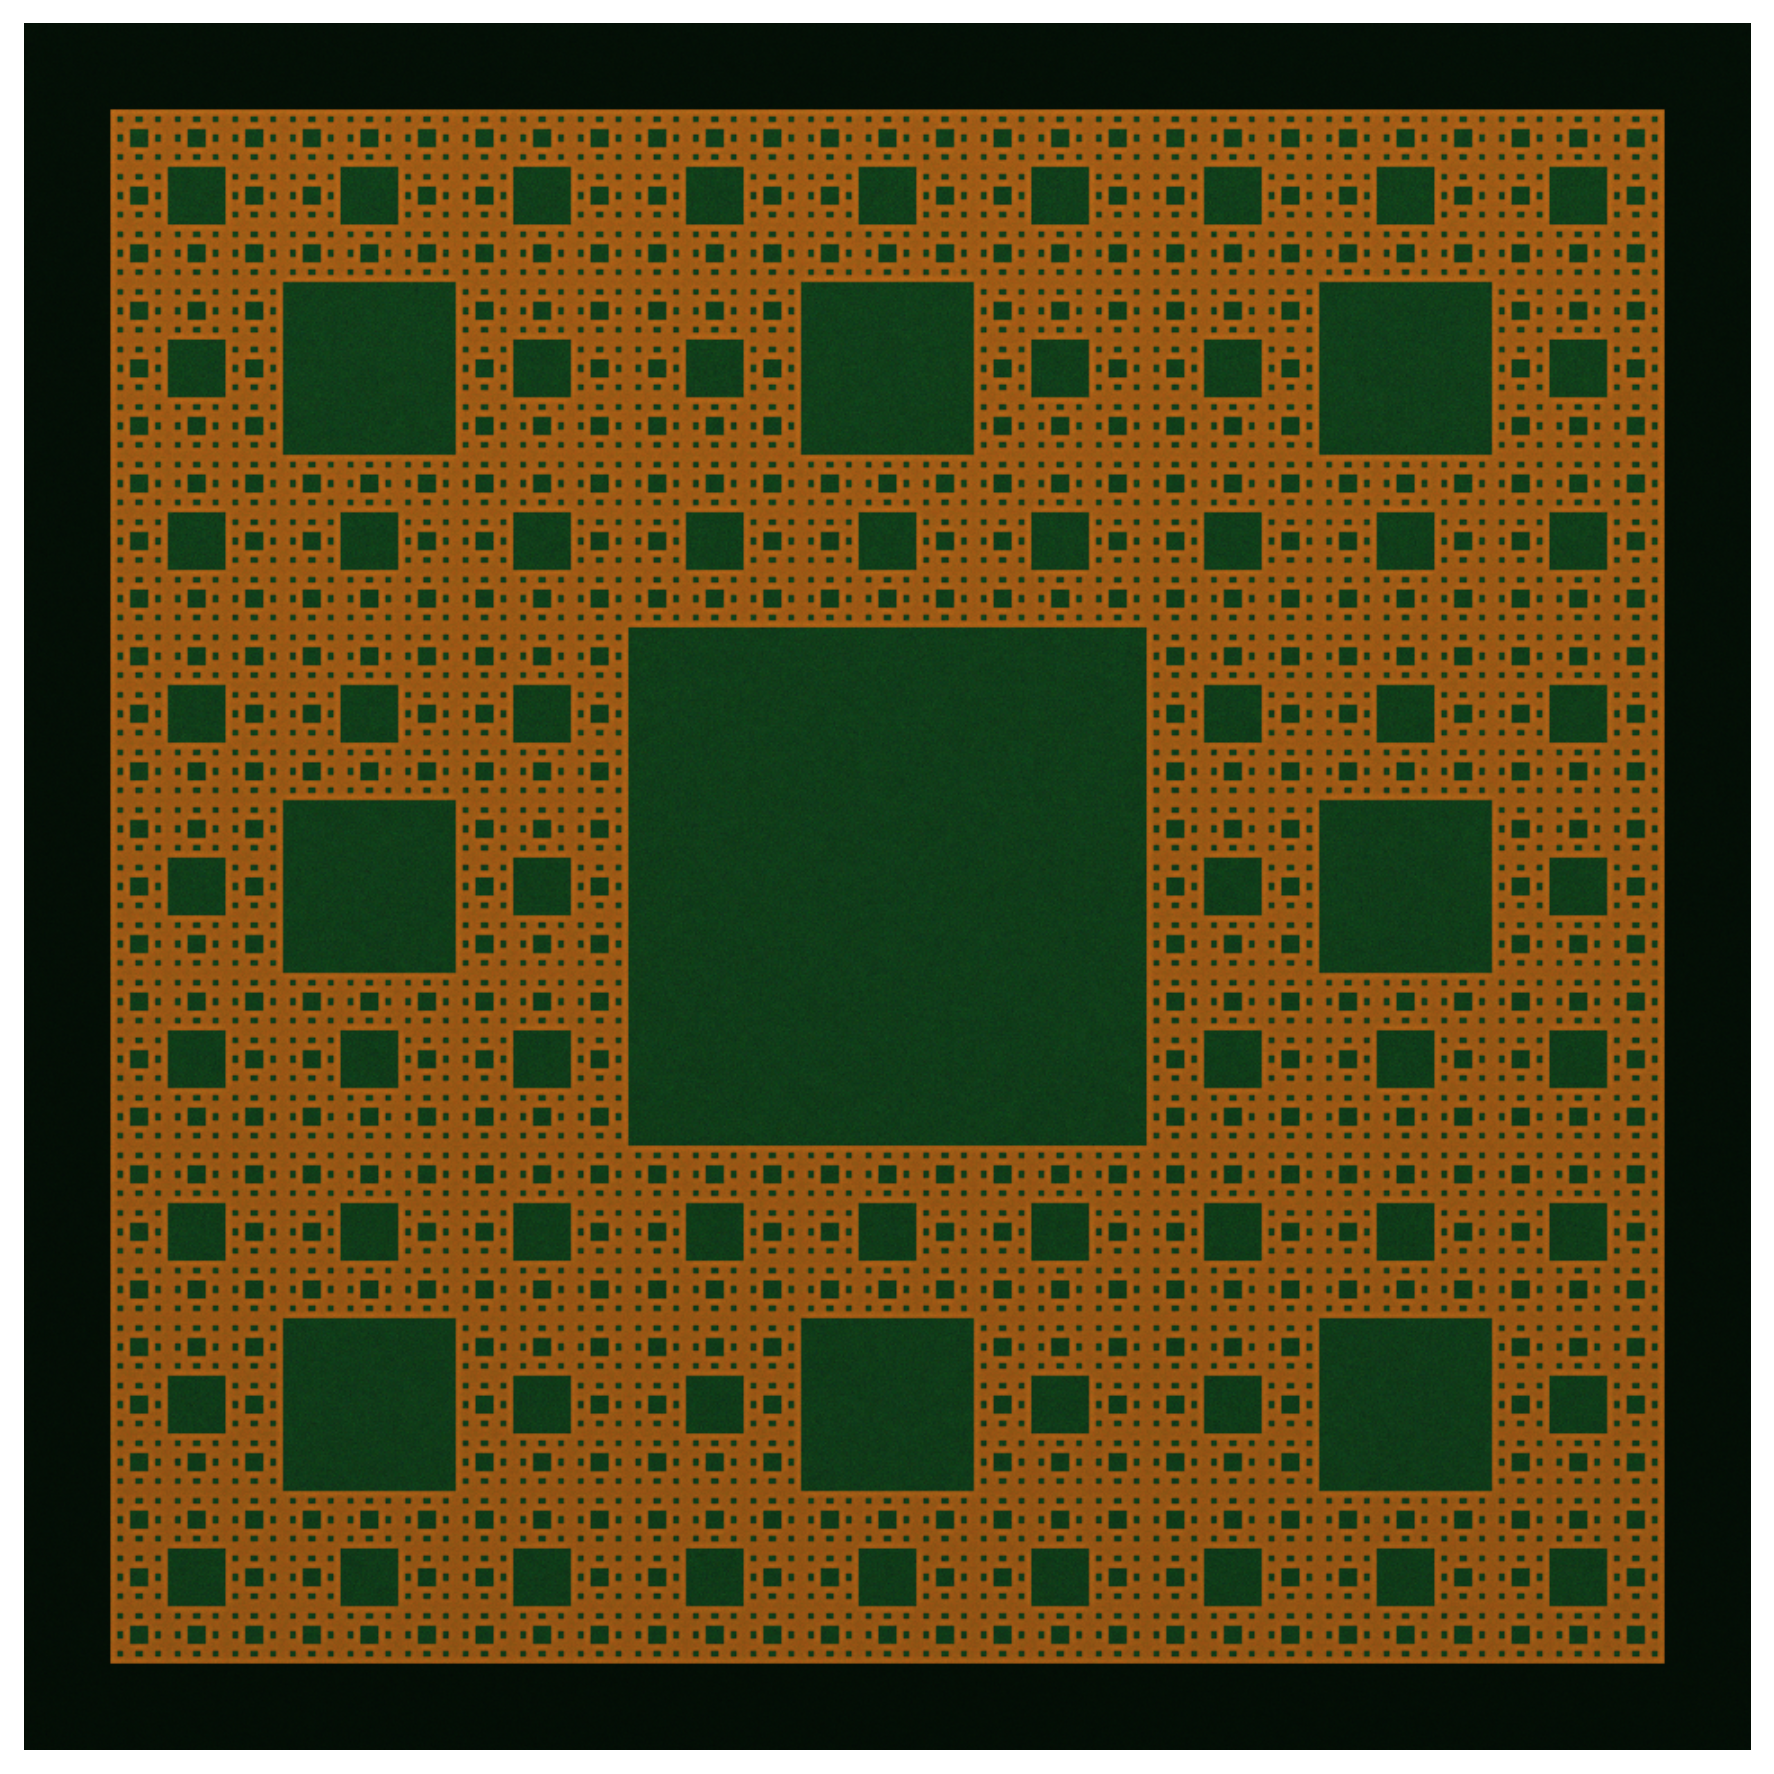
\includegraphics[width=\linewidth,height=0.55\textheight,keepaspectratio]{fig04b_fractal_patch_pcb.png}
  \caption{Планарна патч-антена з фрактальним контуром (\textbf{килим Серпінського}) у міді на зеленій масці лаку: видно самоподібну топологію металізації, характерну для компактних широкосмугових конструкцій\cite{c09,c30}. Зображення --- \textbf{фотореалістичний рендеринг} (імітація макрознімку {PCB}), згенерований скриптом \texttt{generate\_figures.py}, а не патентний кресленик і не скан конкретного заводського зразка.}
  \label{fig:frpatchpcb}
\end{figure}

\begin{figure}[H]
  \centering
  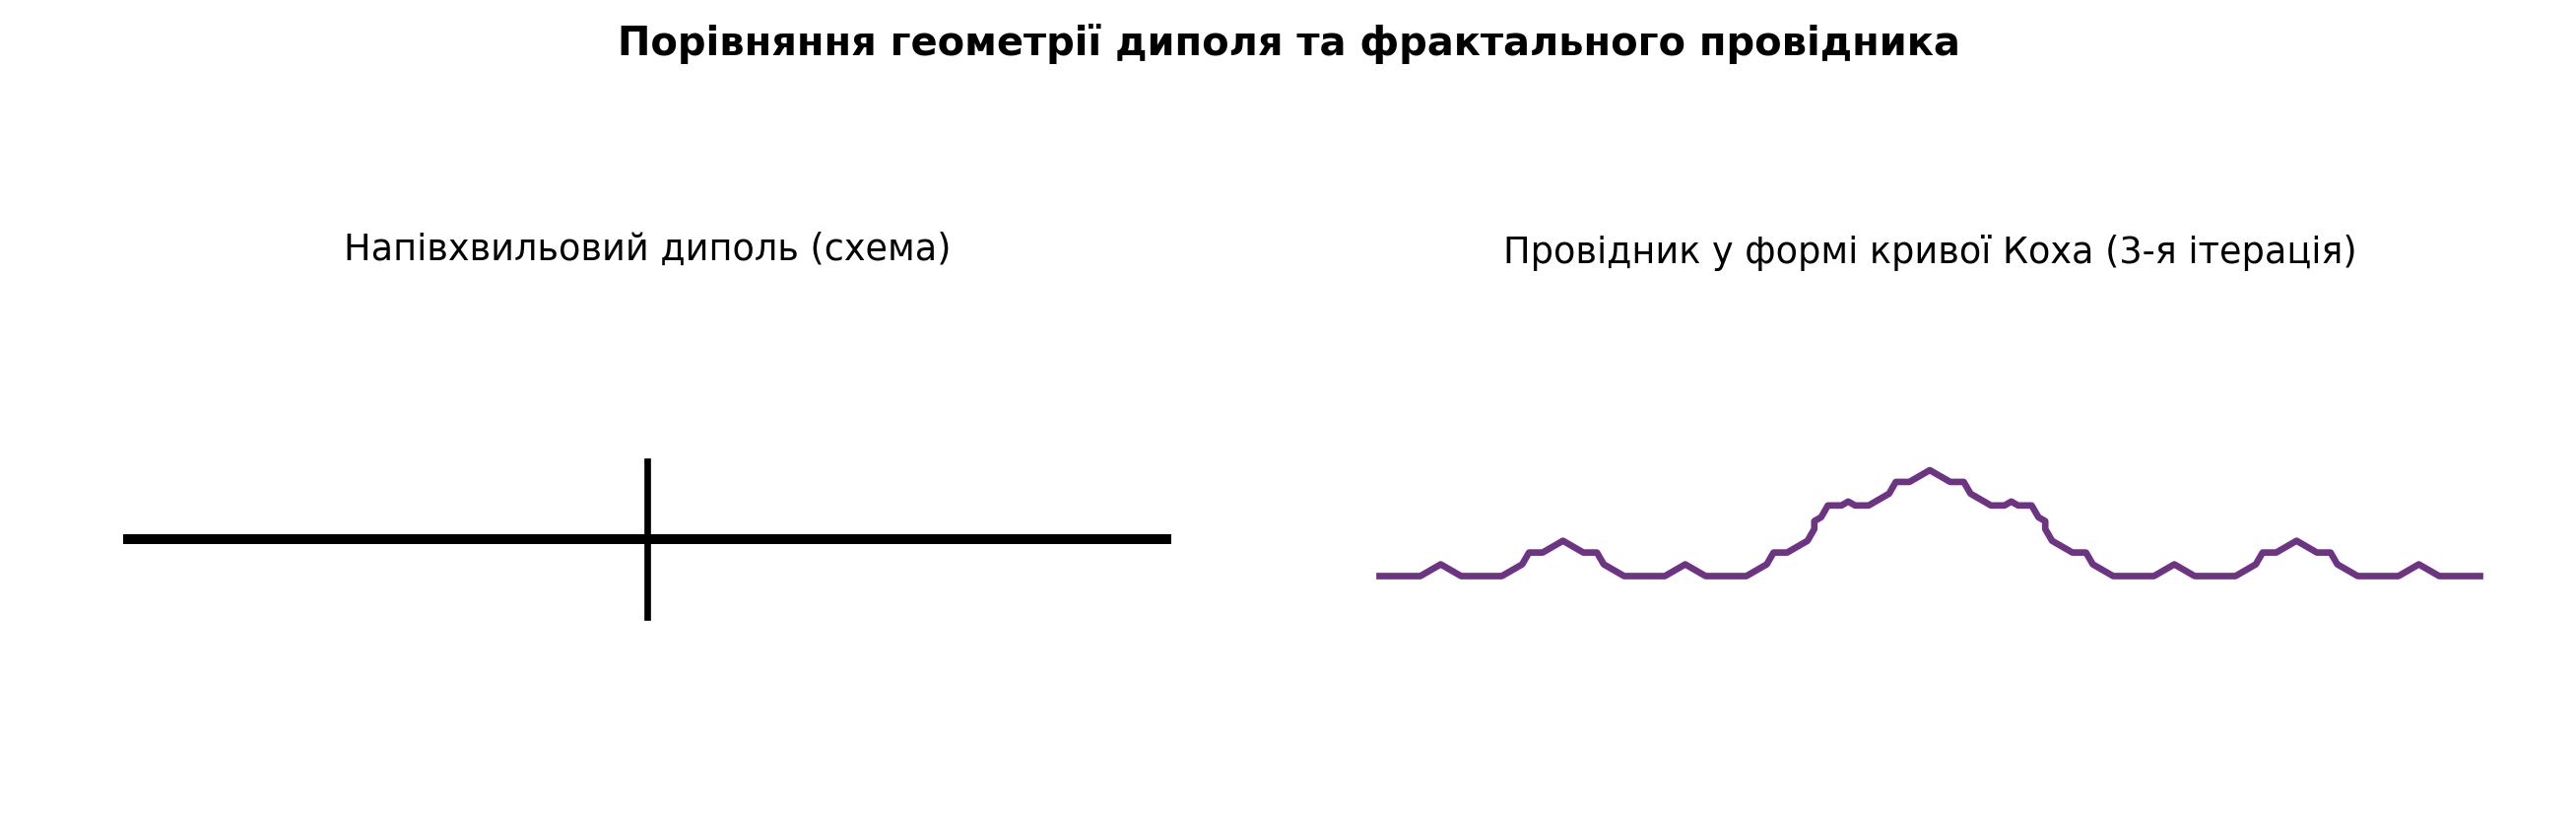
\includegraphics[width=\linewidth]{fig04_antennas.png}
  \caption{Схема напівхвильового диполя та провідника у формі кривої Коха (3-я ітерація) як ілюстрація скорочення габариту.}
  \label{fig:ant}
\end{figure}

\begin{figure}[H]
  \centering
  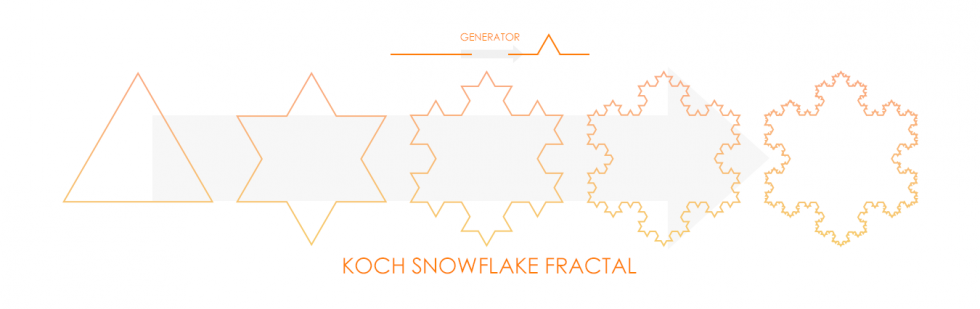
\includegraphics[width=\linewidth,height=0.34\textheight,keepaspectratio]{external/ext_koch.png}
  \caption{Сніжинка Коха (замкнена крива з рекурсивною заміною відрізків): геометрична ілюстрація дробової розмірності довжини контуру. Ілюстрація з блогу {JEM Engineering}\cite{c09}.}
  \label{fig:extkoch}
\end{figure}

\section{Гіпотеза фрактального ринку (FMH) та економічна динаміка}
Класичні гауссівські моделі недооцінюють частоту екстремальних подій; Мандельброт запропонував альтернативу --- FMH.\cite{c06,c13,c33}
Пам'ять ринку описують через показник Херста $H$: $H=0{,}5$ --- броунівський рух; $H>0{,}5$ --- персистентність (тренд); $H<0{,}5$ --- антиперсистентність (реверсія до середнього).\cite{c13,c33,c06}
Стабільність «фрактального ринку» пов'язують із різноманіттям інвестиційних горизонтів; уніфікація коротких горизонтів підсилює ризик ламання структури.\cite{c13}
Сучасний аналіз волатильності та «товстих хвостів» опирається на фрактальні та мультифрактальні методи.\cite{c35,c34,c06}

\begin{figure}[H]
  \centering
  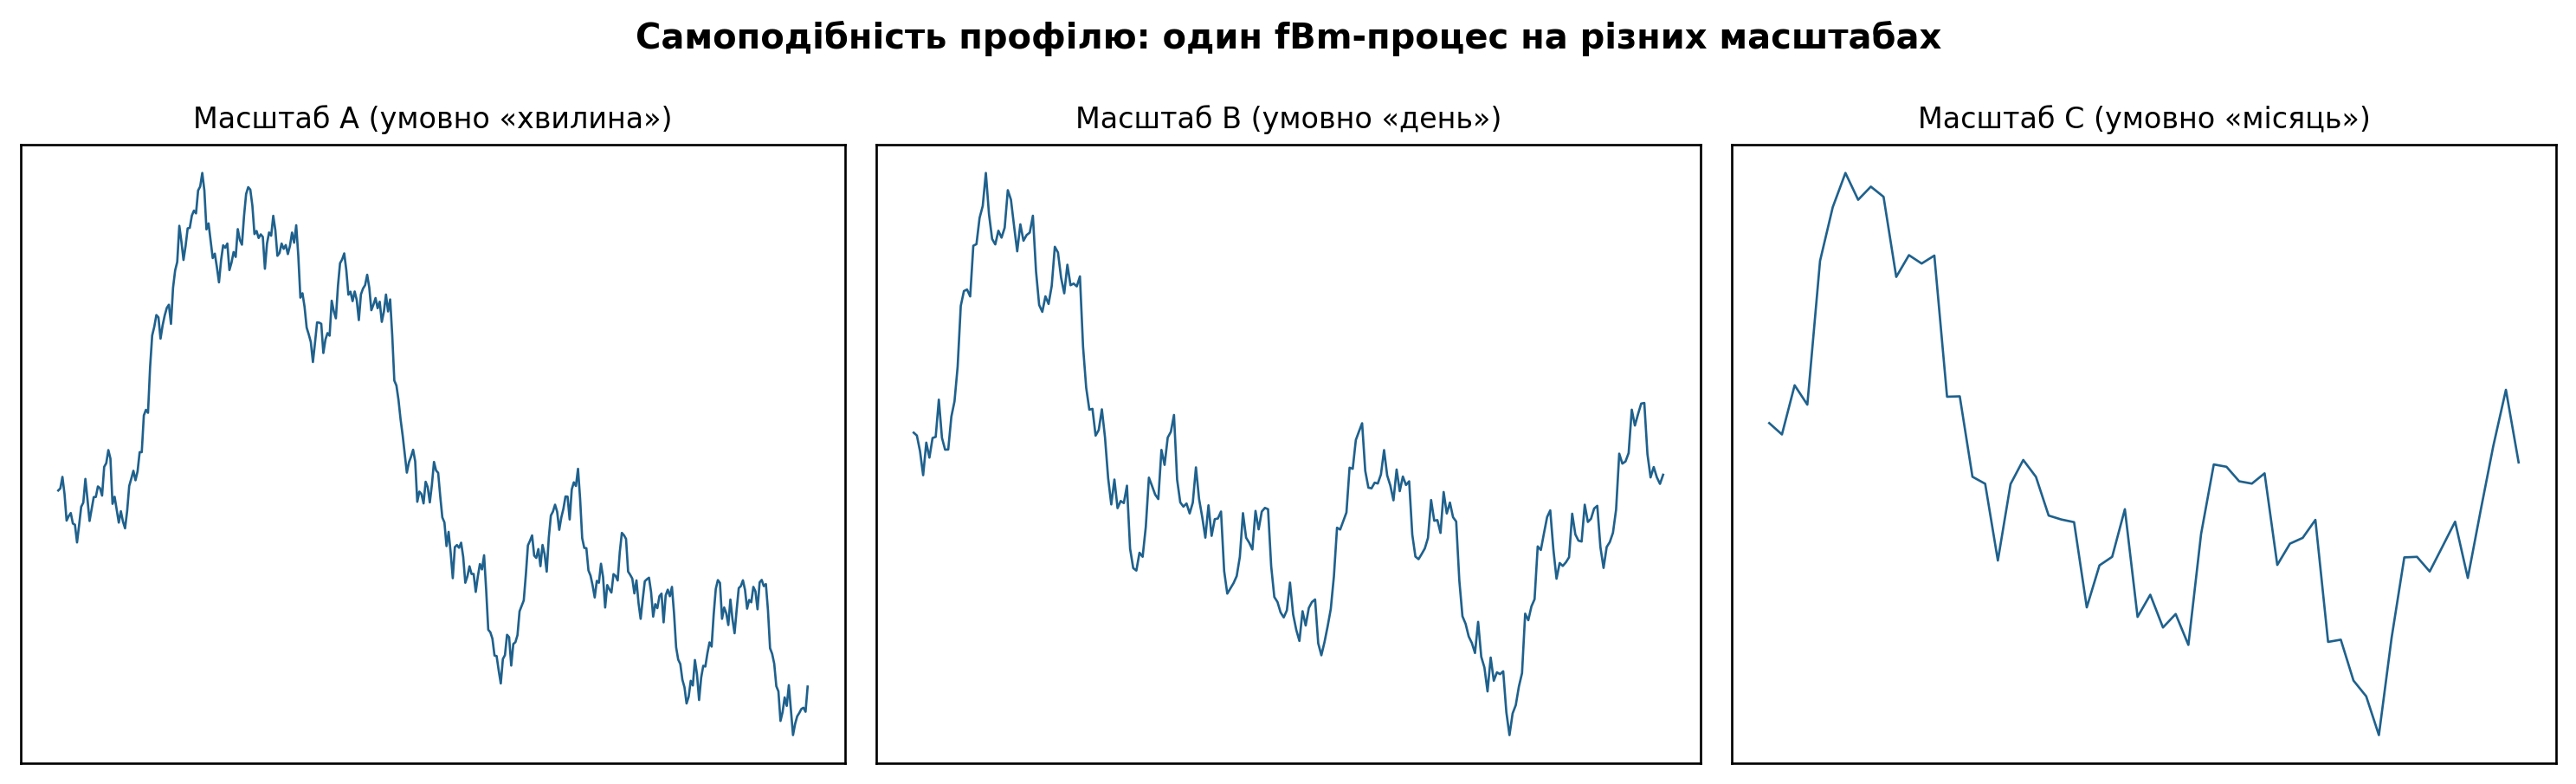
\includegraphics[width=\linewidth]{fig05_finance_scales.png}
  \caption{Три масштаби одного самоподібного синтетичного профілю (наближення до ідеї «хвилина / день / місяць»).}
  \label{fig:fin}
\end{figure}

\section{Дифузійно-обмежена агрегація (DLA)}
DLA (Witten---Sander, 1981) моделює частинку-«насіння», броунівський рух нових частинок і прилипання при контакті з кластером.\cite{c37,c38,c36}
Застосування: дендритна кристалізація, геологічні дендрити, електричний пробій, блискавка; у техніці --- пористі середовища, охолодження мікросхем, поширення забруднень.\cite{c37,c39,c24}

\begin{figure}[H]
  \centering
  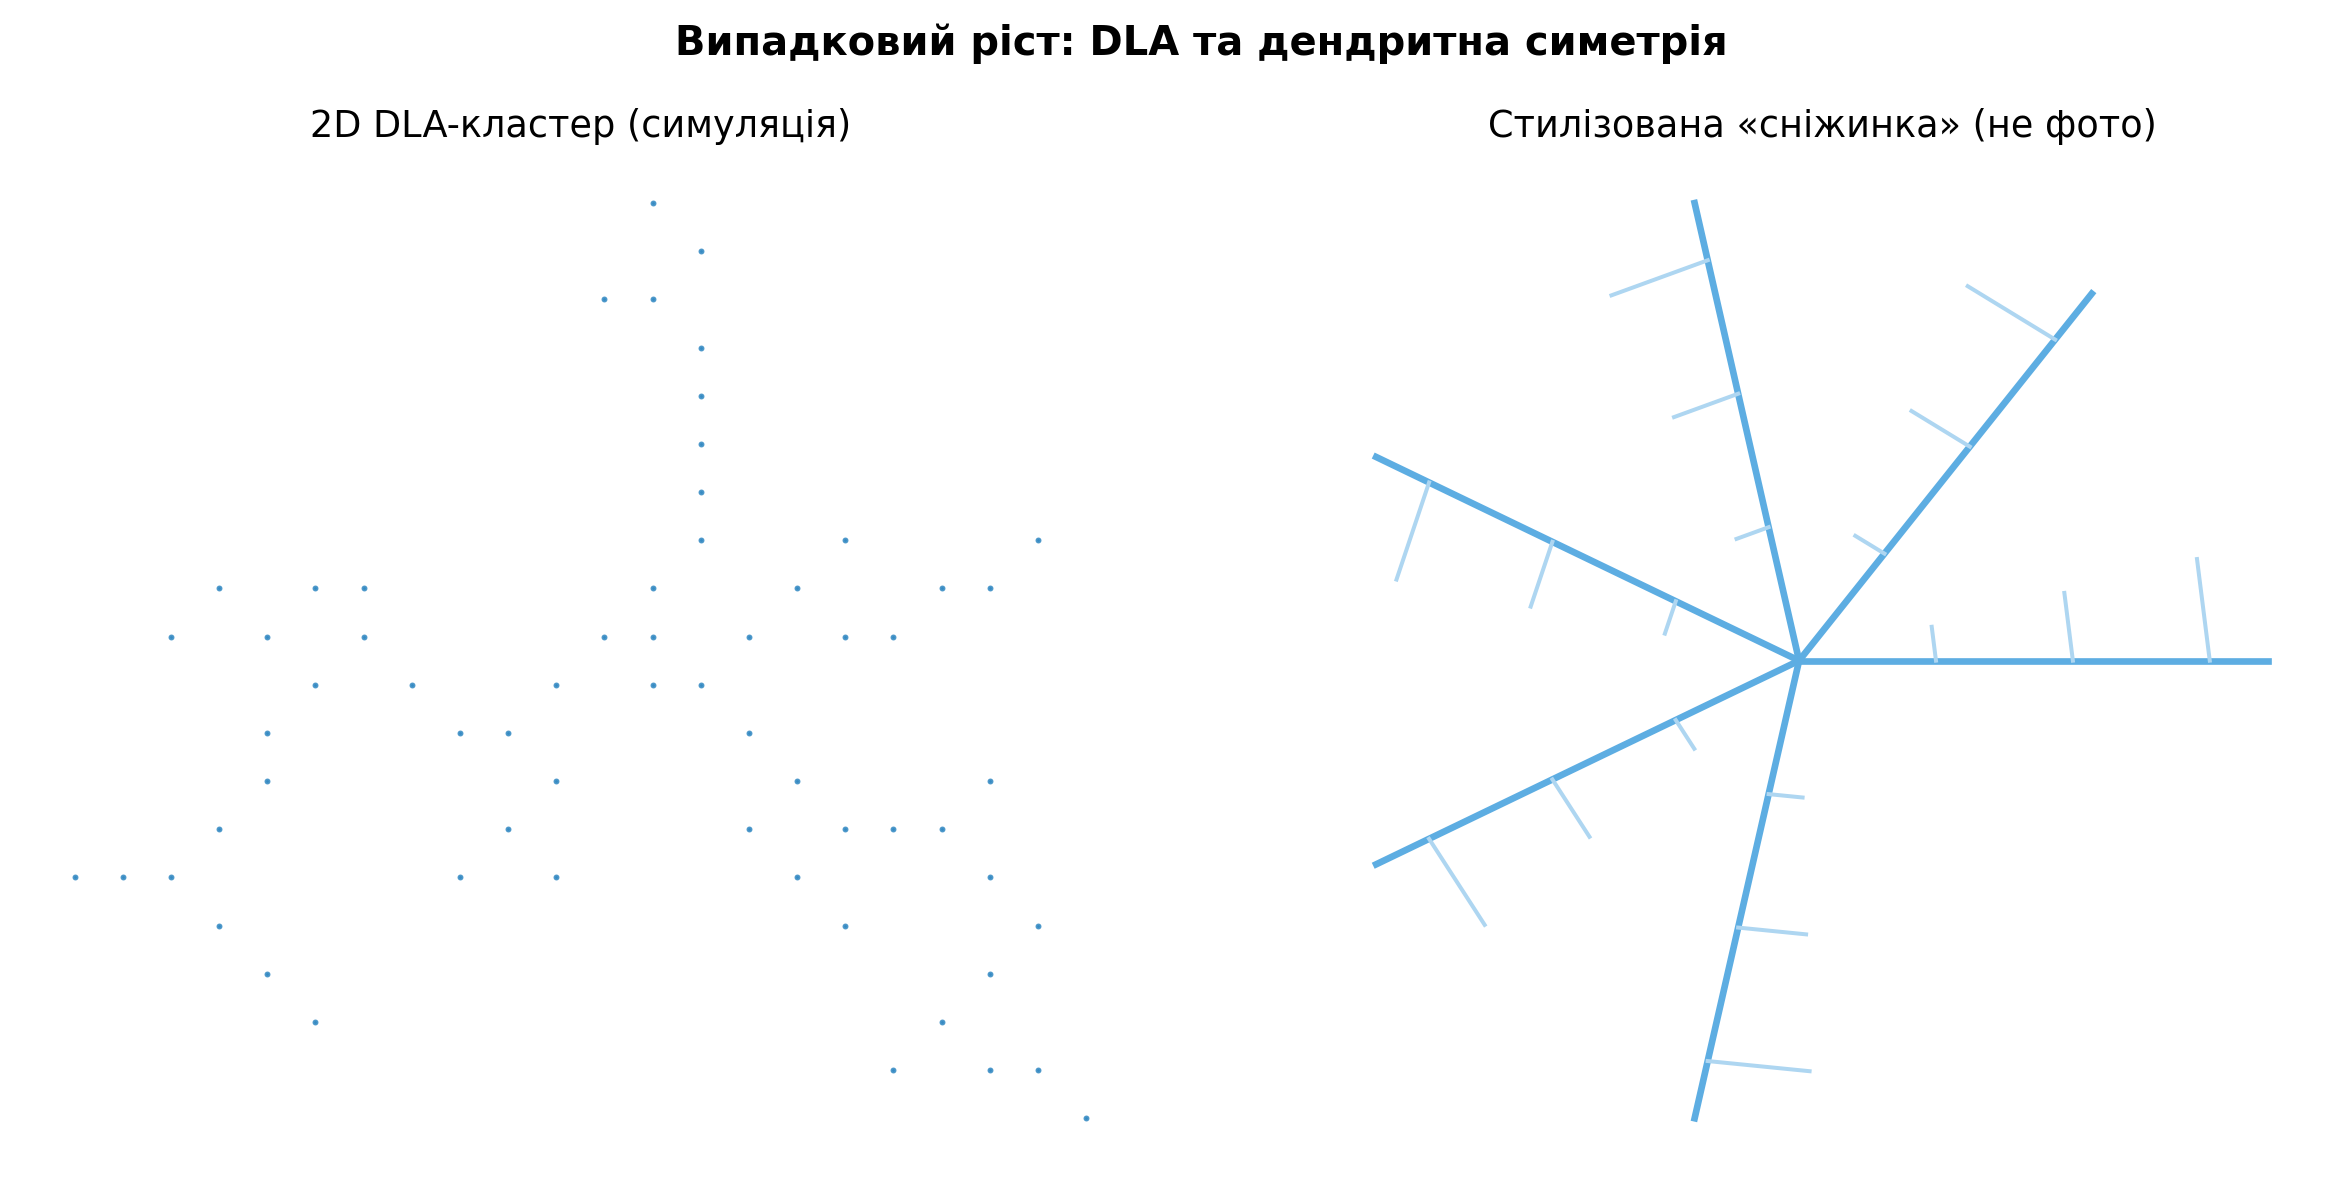
\includegraphics[width=\linewidth]{fig06_dla_snowflake.png}
  \caption{2D DLA-кластер (симуляція) та стилізована «сніжинка»; літературна оцінка $D\approx 1{,}71$ для 2D DLA наводиться як орієнтир\cite{c37,c38}, а не як результат цього малого кластера.}
  \label{fig:dla}
\end{figure}

\section{Стохастичний фрактальний пошук (SFS)}
Алгоритм SFS (Salimi, 2015) поєднує фазу «дифузії» (генерація нових точок навколо кандидатів) і фазу оновлення зі стохастичними природними евристиками.\cite{c40}
Застосовують у енергетиці (smart grid), бездротових сенсорних мережах, навчанні нейромереж.\cite{c40}

\begin{figure}[H]
  \centering
  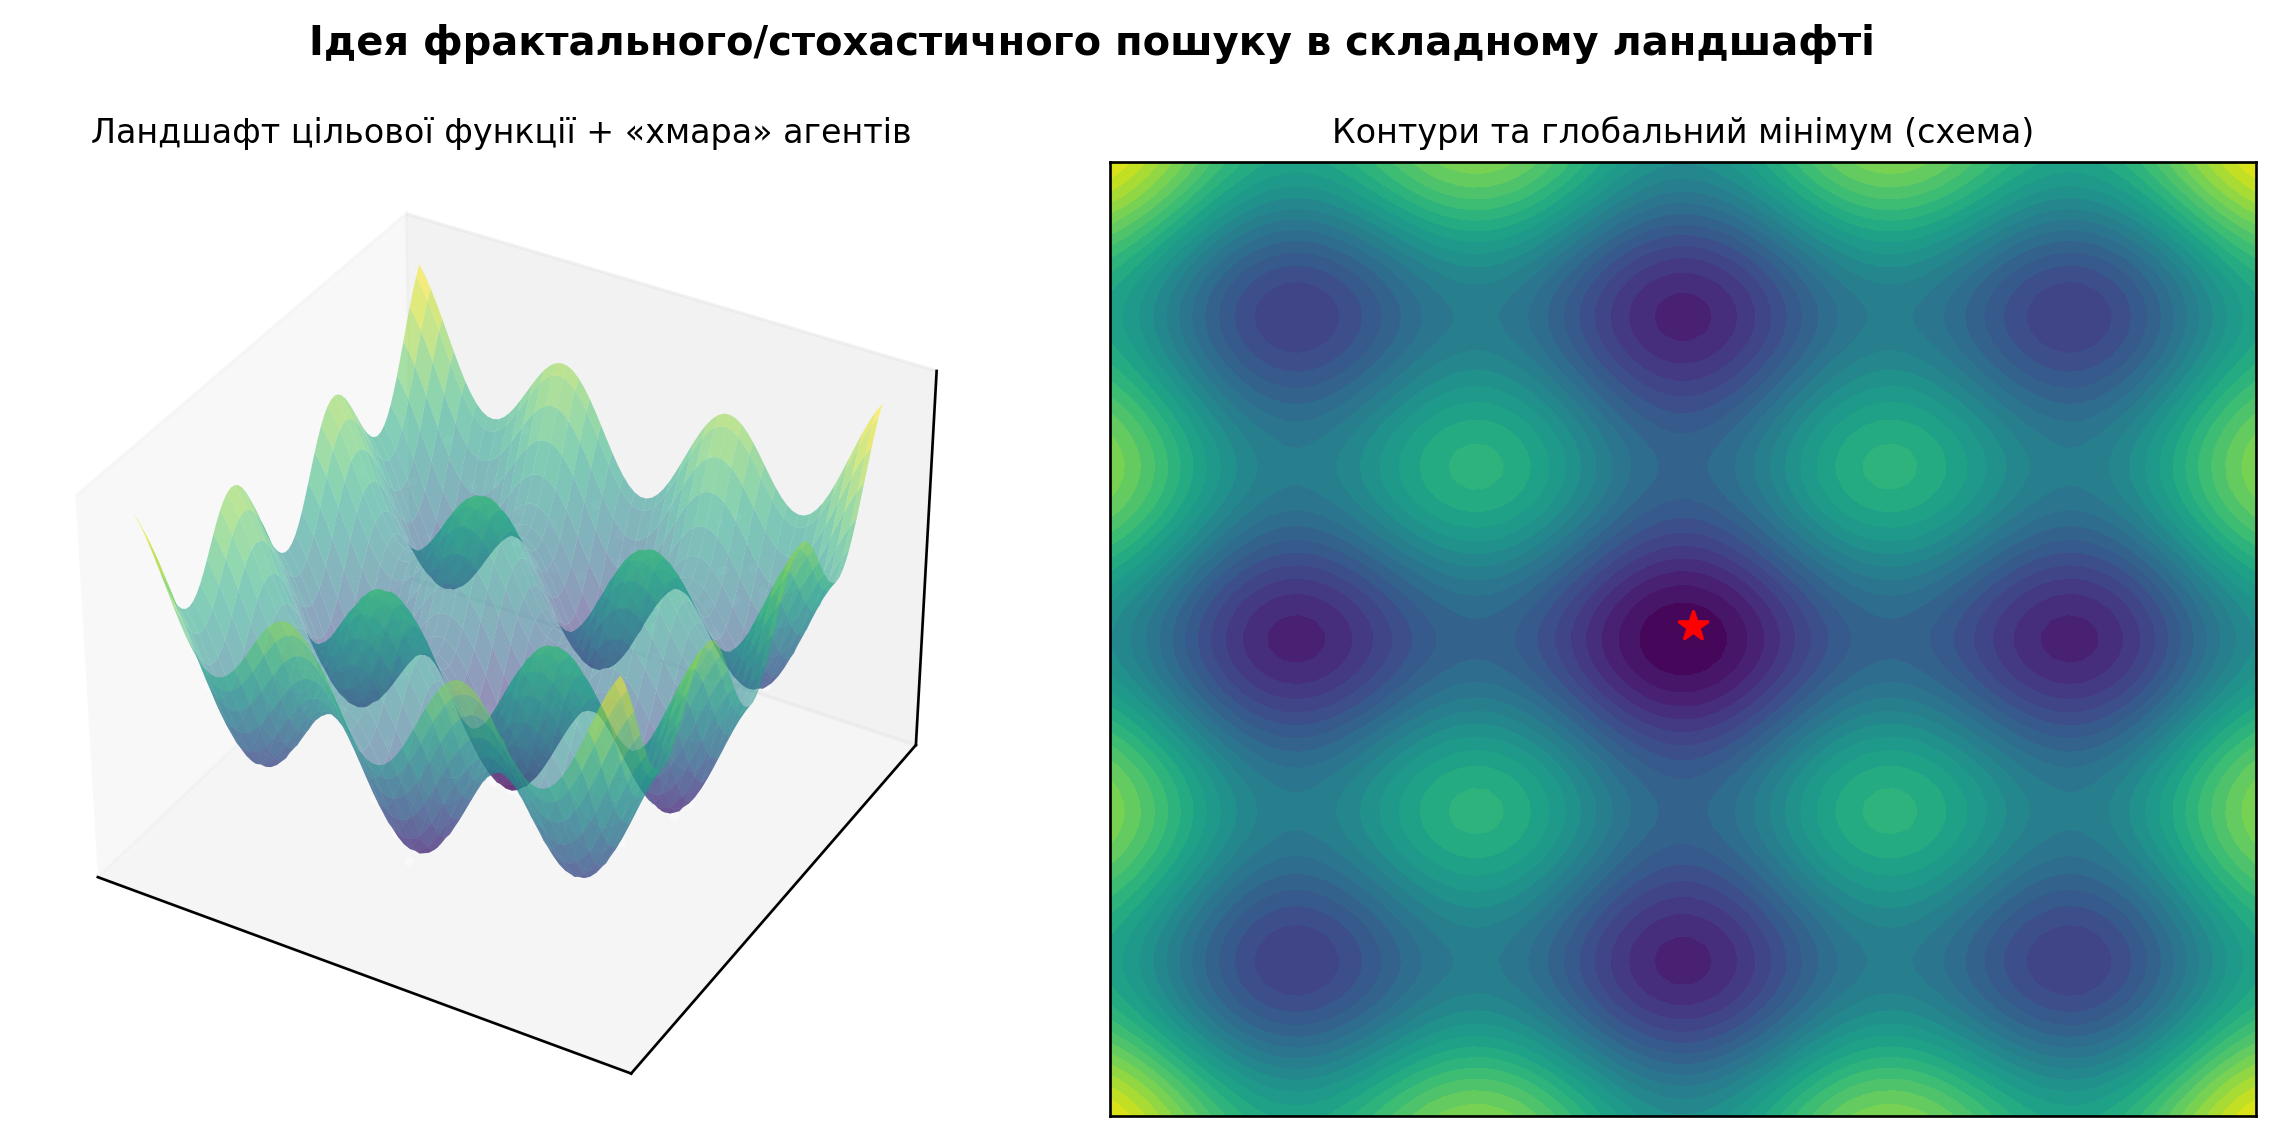
\includegraphics[width=\linewidth]{fig07_sfs.png}
  \caption{Ландшафт цільової функції з локальними мінімумами та «хмара» точок-агентів (навчальна схема).}
  \label{fig:sfs}
\end{figure}

\section{Метеорологія та екологічний моніторинг}
Турбулентна атмосфера демонструє масштабну самоподібність; фрактальні методи застосовують до супутникових даних (класифікація хмар, опади), аналізу нічного освітлення міст.\cite{c41,c42,c43,c44}
Ріст міст можна трактувати як стохастичний фрактальний процес порівняно з регулярними сітками.\cite{c01}

\begin{figure}[H]
  \centering
  \resizebox{\linewidth}{!}{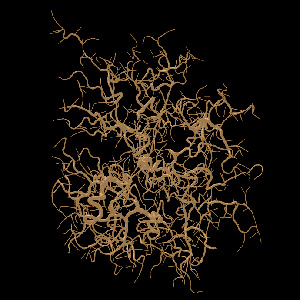
\includegraphics{external/ext_hurricane.jpg}}
  \caption{Двовимірний {DLA}-кластер з точковим атрактором (класична симуляція): у літературі наводять аналогії з дендритним ростом і гілкуванням блискавки. {Paul Bourke}\cite{c38}.}
  \label{fig:extdla}
\end{figure}

\begin{figure}[H]
  \centering
  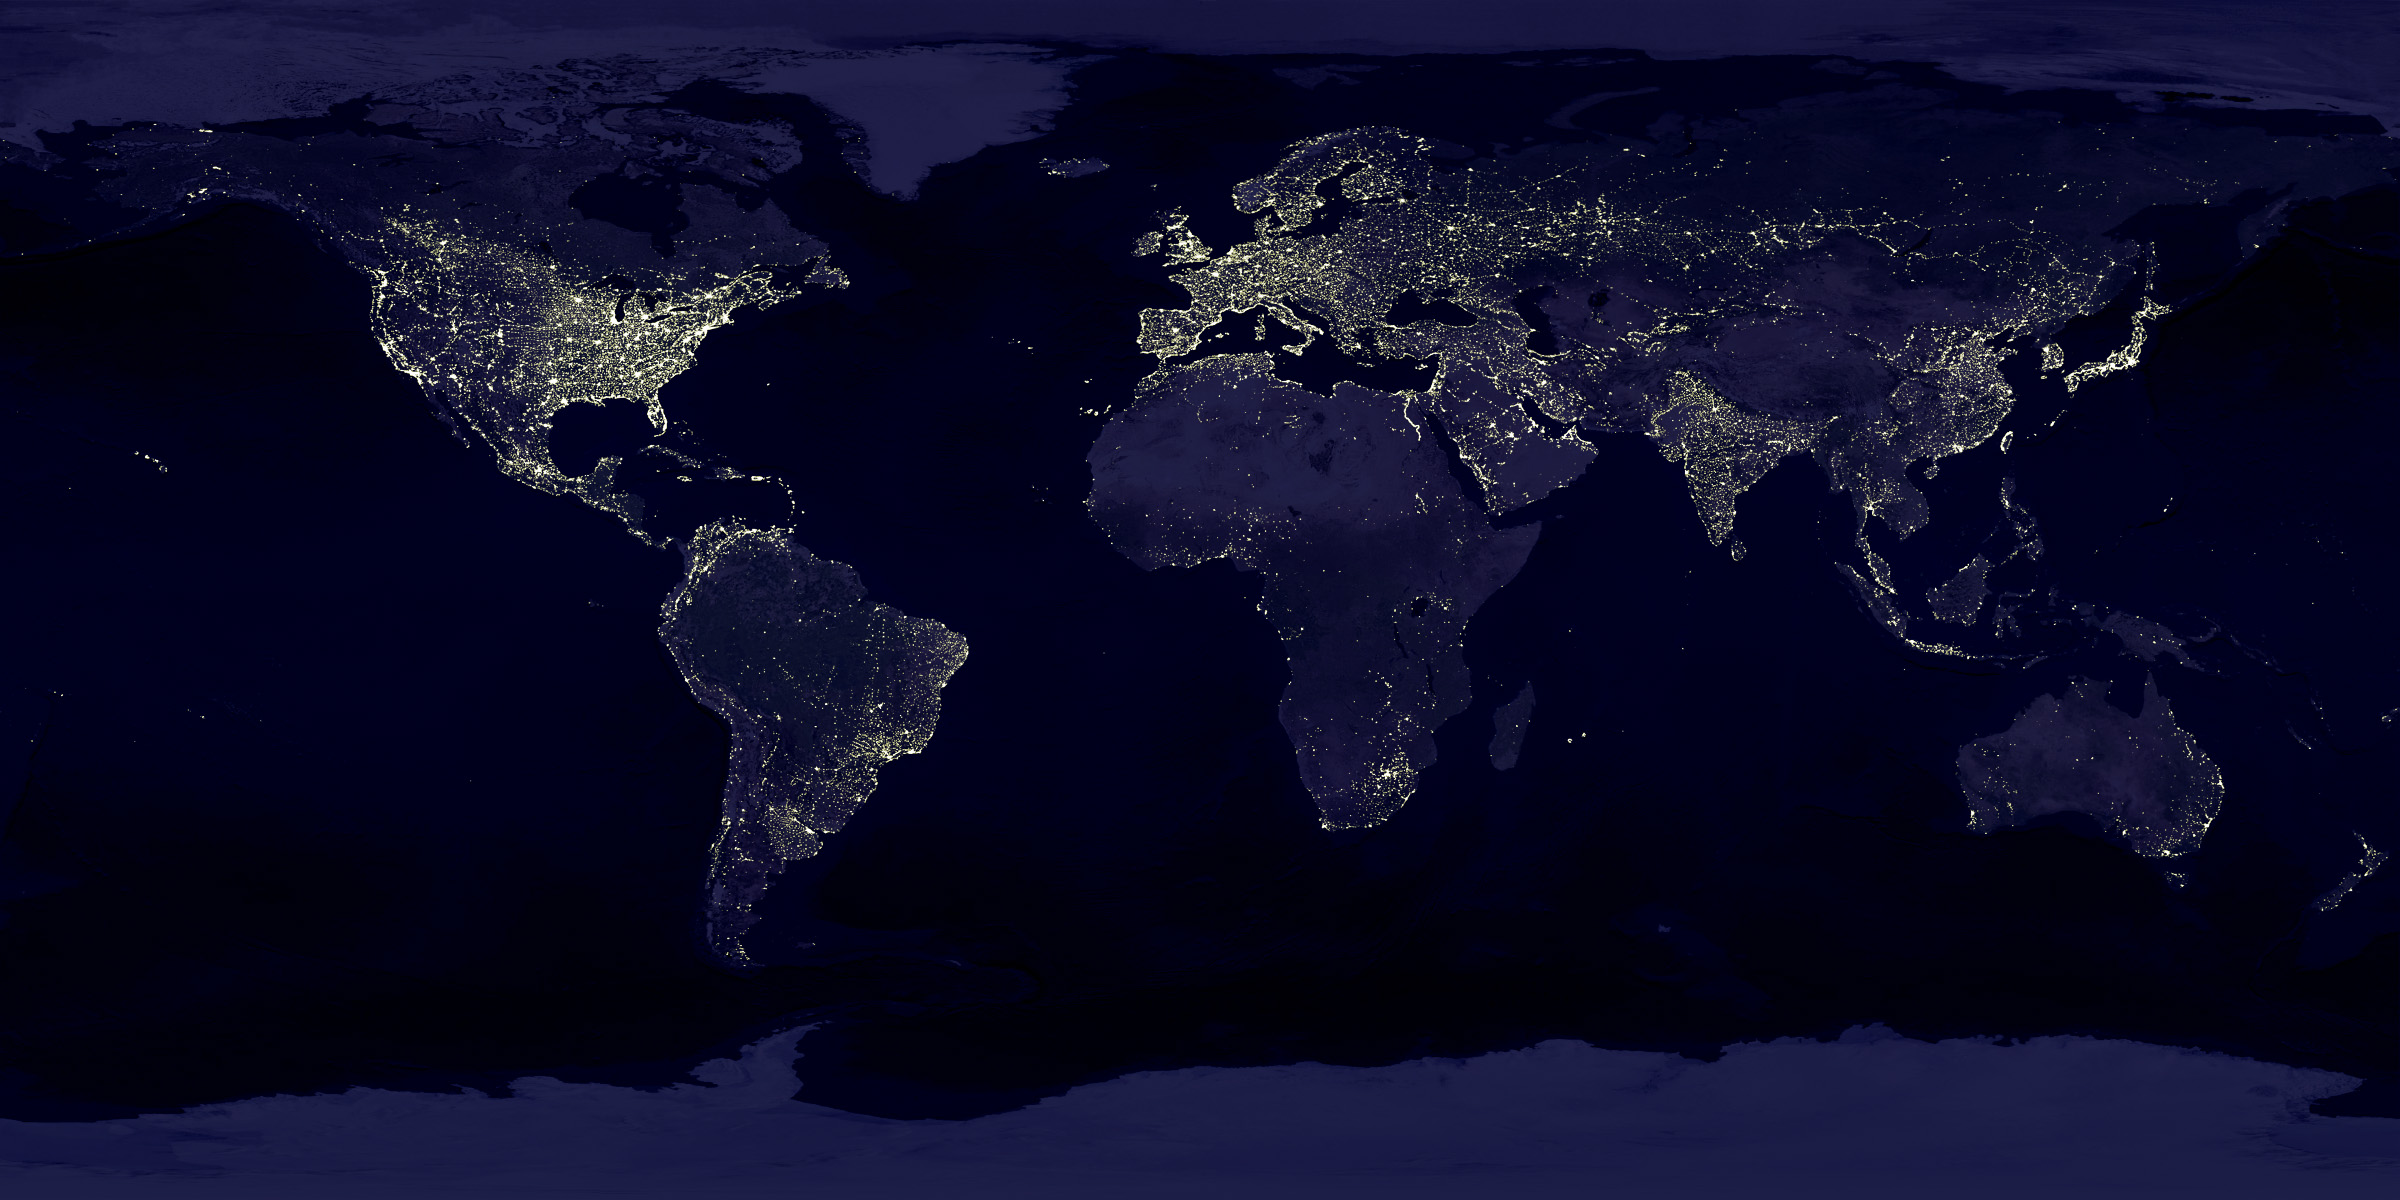
\includegraphics[width=\linewidth]{external/ext_earthlights.jpg}
  \caption{Земля вночі (композит штучного освітлення): агреговане поле яскравості як основа для аналізу просторової структури урбанізації. {NASA} {Earth} {Observatory} / {GSFC}\cite{c52}.}
  \label{fig:extnight}
\end{figure}

\begin{figure}[H]
  \centering
  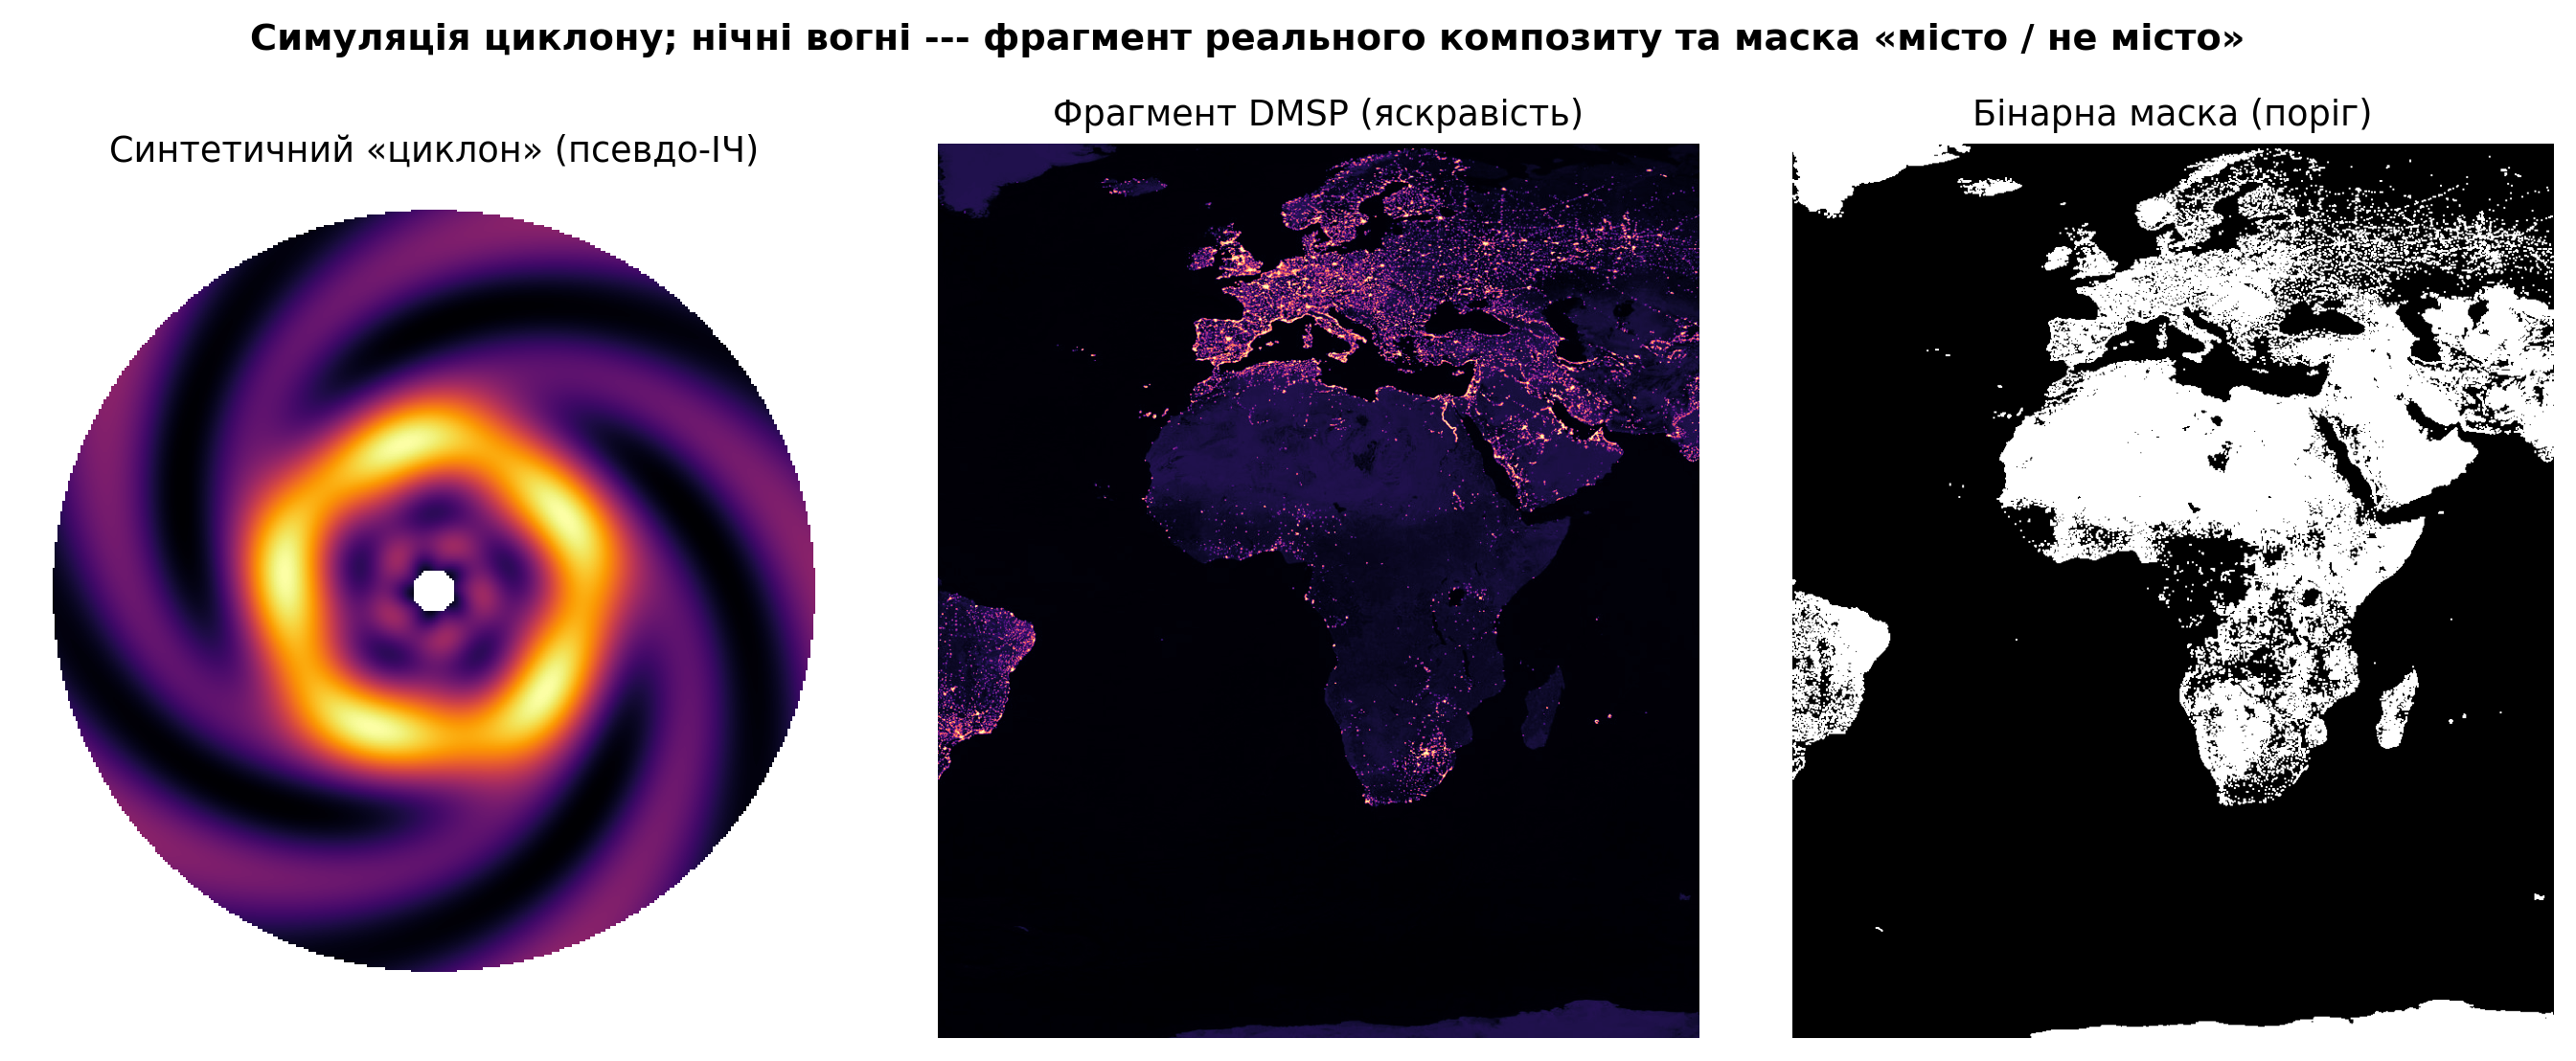
\includegraphics[width=\linewidth]{fig08_cyclone_night.png}
  \caption{Ліворуч --- синтетичне поле інтенсивності (псевдо-ІЧ): модель ока та спіральних смуг; у центрі та праворуч --- збільшений фрагмент того самого композиту нічних вогнів, що на рис.~\ref{fig:extnight} (яскравість і бінарна маска після порога для виділення освітлених територій і нерегулярної межі агломерації).}
  \label{fig:met}
\end{figure}

\section{Висновки}
Стохастичні фрактали еволюціонували від математичної абстракції до інженерного інструментарію: мініатюризація антен, медична діагностика за FD, стійкіші фінансові моделі, процедурна графіка та стиснення зображень.\cite{c24,c06,c09}
Перспектива --- мультифрактальний аналіз із спектром показників замість одного $D$.\cite{c35,c15}

\bibliographystyle{unsrtnat}
\bibliography{referat}

\end{document}
